\documentclass[preprint,12pt,aps,pra,showkeys,amsmath,amssymb,superscriptaddress,floatfix]{revtex4-2}
\usepackage[T1]{fontenc}
\usepackage[utf8]{inputenc}
\usepackage{amsmath,amssymb,amsthm,mathtools,mathrsfs}
\usepackage{microtype,booktabs,enumitem}
\usepackage{xcolor,tikz,etoolbox}
\usepackage[skins,breakable]{tcolorbox}
\usepackage{needspace}
% Keep diagram geometry independent of REVTeX preprint body spacing.
\AtBeginEnvironment{tikzpicture}{\linespread{1}\selectfont}
\usetikzlibrary{arrows.meta,positioning,calc,fit,decorations.pathreplacing}
\usepackage{graphicx}
\usepackage{hyperref}

\definecolor{MMBlue}{RGB}{0,82,155}
\definecolor{MMOrange}{RGB}{200,80,0}
\tikzset{
 mmnode/.style={draw=MMBlue,rounded corners=2pt,fill=MMBlue!4,align=left,execute at begin node={\raggedright},text width=5cm,font=\fontsize{10}{12}\selectfont,inner sep=6pt},
 mmimport/.style={mmnode,draw=black!65,fill=black!4},
 mmcandidate/.style={mmnode,draw=MMOrange,dashed,fill=MMOrange!5},
 mmrejected/.style={mmnode,draw=black,densely dotted,fill=black!8},
 mmproof/.style={->,thick,MMBlue},
 mmflow/.style={->,semithick,black!70},
 mmrepair/.style={->,dashed,thick,MMOrange},
 mmcandidatearrow/.style={->,dashed,semithick,MMOrange},
 mmnote/.style={font=\scriptsize,fill=white,inner sep=2pt,align=center}}

\usepackage[section]{placeins}
\setlength{\emergencystretch}{3em}
\setlist{itemsep=3pt,topsep=4pt}
\newtheorem{theorem}{Theorem}[section]
\newtheorem{proposition}[theorem]{Proposition}
\newtheorem{lemma}[theorem]{Lemma}
\newtheorem{corollary}[theorem]{Corollary}
\theoremstyle{definition}
\newtheorem{definition}[theorem]{Definition}
\newtheorem{example}[theorem]{Example}
\theoremstyle{remark}
\newtheorem{remark}[theorem]{Remark}
% Avoid isolated statement headings and single-line paragraph fragments.
\BeforeBeginEnvironment{theorem}{\Needspace{6\baselineskip}}
\BeforeBeginEnvironment{definition}{\Needspace{5\baselineskip}}
\BeforeBeginEnvironment{proposition}{\Needspace{5\baselineskip}}
\BeforeBeginEnvironment{lemma}{\Needspace{5\baselineskip}}
\BeforeBeginEnvironment{corollary}{\Needspace{5\baselineskip}}
\clubpenalty=5000
\widowpenalty=5000
\newcommand{\R}{\mathbb R}\newcommand{\Z}{\mathbb Z}\newcommand{\N}{\mathbb N}
\newcommand{\Pa}{\operatorname{Pa}}\newcommand{\Desc}{\operatorname{Desc}}
\newcommand{\cl}{\operatorname{cl}}\newcommand{\cost}{\operatorname{cost}}
\newcommand{\status}{\operatorname{status}}
% Faculty cards: a visual rail groups the five faculties within one agent.
% The rail has no arrowhead and does not represent a proof dependency.
\newcommand{\mmfacultybadge}[1]{%
 \node[circle,draw=MMBlue,line width=1pt,fill=white,
 minimum size=7mm,inner sep=0pt,font=\sffamily\small\bfseries,text=MMBlue]
 at ([xshift=15pt,yshift=-15pt]frame.north west) {#1};}
\newcommand{\mmfacultyrail}{%
 \draw[MMBlue!80,line width=1pt]
 ([xshift=15pt,yshift=2pt]frame.north west)--
 ([xshift=15pt,yshift=-2pt]frame.south west);}
\newtcolorbox{mmfacultybox}[2]{enhanced,breakable,
 colback=MMBlue!4,colframe=MMBlue!4,boxrule=0pt,arc=3pt,
 left=39pt,right=9pt,top=4pt,bottom=4pt,
 before skip=2pt,after skip=2pt,
 fontupper=\small\linespread{1.1}\selectfont,
 overlay unbroken={\mmfacultyrail\mmfacultybadge{#1}},
 overlay first={\mmfacultyrail\mmfacultybadge{#1}},
 overlay middle={\mmfacultyrail},overlay last={\mmfacultyrail}}
\newcommand{\mmfaculty}[3]{%
 \begin{mmfacultybox}{#1}{#2}
 {\sffamily\bfseries\color{MMBlue}#2}\par\smallskip #3
 \end{mmfacultybox}}
\newcommand{\agent}[9]{%
 \Needspace{8\baselineskip}
 \subsubsection{#1}
 \noindent\textbf{Object.} #2\par
 \noindent\textbf{Role.} #3\par\smallskip
 \mmfaculty{E}{Ego}{#4}
 \mmfaculty{M}{Memory}{#5}
 \mmfaculty{I}{Intellect}{#6}
 \mmfaculty{S}{Sense}{#7}
 \mmfaculty{A}{Action}{#8}
 \smallskip\noindent #9\par}

\usepackage{longtable,array,calc}
\providecommand{\tightlist}{\setlength{\itemsep}{2pt}\setlength{\parskip}{0pt}}
\makeatletter
\def\frontmatter@abstract@produce{\par\addvspace{\frontmatter@preabstractspace}%
\begingroup\prep@absbox\unvbox\absbox\post@absbox\endgroup
\addvspace{\frontmatter@postabstractspace}}
\makeatother
\newcommand{\field}[2]{\par\smallskip\noindent\textbf{#1.} #2\par}
\setlength{\emergencystretch}{5em}
\AtBeginEnvironment{verbatim}{\small\linespread{1.0}\selectfont}


\hypersetup{colorlinks=true,linkcolor=MMBlue,urlcolor=MMBlue,pdfauthor={Dibakar Sigdel}}

\begin{document}

\title{Classification of Groups of Order pq\\[4pt]\large An End-to-End Meta-Math Walkthrough}

\author{Dibakar Sigdel}

\affiliation{Mindverse Computing LLC, Lynnwood, WA 98087, USA}

\date{October 2026}

\begin{abstract}

A complete authored walkthrough of classification of groups of order pq,
with explicit mathematical contracts, local verification gates, and
reusable exports. The report presents the target theorem, declared
imports, a dependency graph, five-faculty node contracts, a continuous
proof, a worked example, and a hypothesis-repair audit. It is an
authored mathematical exposition, not a deployed-agent transcript or a
formal proof-assistant certificate.

\end{abstract}\maketitle\linespread{1.12}\selectfont

\noindent\textbf{MA-03 / Modern Algebra / Report v1}

\section{Target and import contract}

\begin{theorem}

Let \(p<q\) be primes. If p does not divide \(q-1\), every group of
order pq is isomorphic to \(C_{pq}\). If p divides \(q-1\), there are
exactly two isomorphism classes: \(C_{pq}\) and one nonabelian group
\(C_q\rtimes C_p\).

A complete classification must prove that every input group has one of
the stated structures, construct each listed structure, and prove that
apparently different nontrivial constructions are isomorphic. Sylow
congruences alone do not close these obligations.

\end{theorem}

\subsection{Foundations and permitted imports}

Sylow's existence/counting theorems; Lagrange's theorem; finite
product-set counting; the theorem that the multiplicative group of the
prime field \(F_q\) is cyclic of order \(q-1\). The last result is the
supporting primitive-root module, not an unstated assumption.
Prime-order groups are cyclic because a nonidentity element generates a
subgroup whose nontrivial order divides that prime.

\clearpage\section{Node interaction workflow}

\begin{center}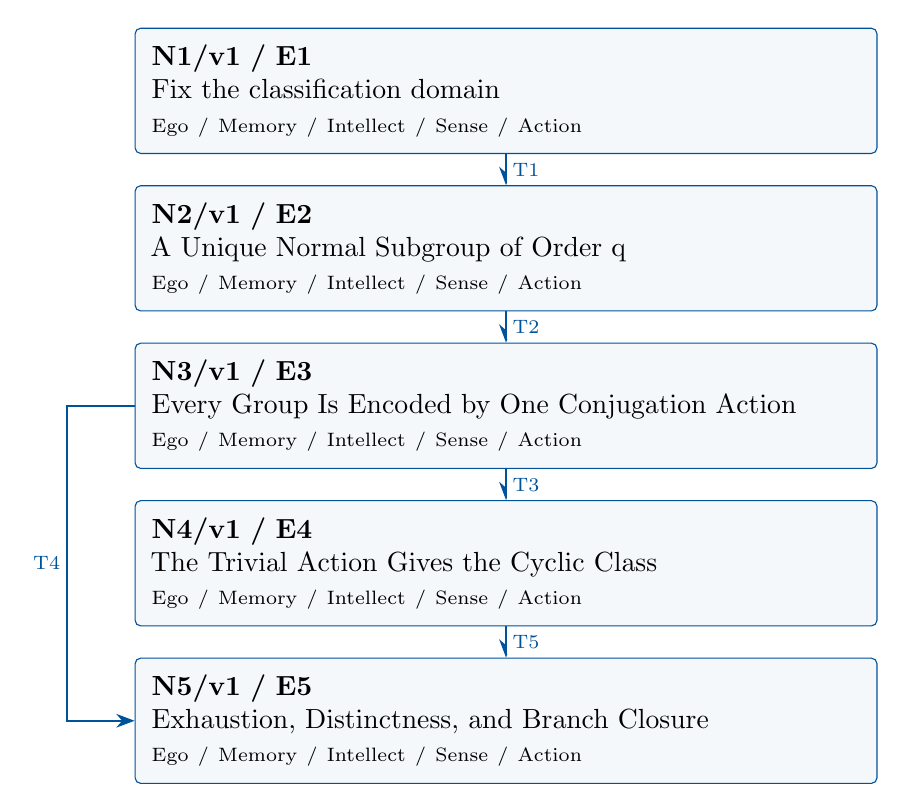
\begin{tikzpicture}[>=Stealth,x=1cm,y=1cm]

\node[mmnode,text width=9cm,minimum height=1.25cm] (N1) at (0,0.0) {\textbf{N1/v1 / E1}\\Fix the classification domain\\{\scriptsize Ego / Memory / Intellect / Sense / Action}};

\node[mmnode,text width=9cm,minimum height=1.25cm] (N2) at (0,-2.0) {\textbf{N2/v1 / E2}\\A Unique Normal Subgroup of Order q\\{\scriptsize Ego / Memory / Intellect / Sense / Action}};

\node[mmnode,text width=9cm,minimum height=1.25cm] (N3) at (0,-4.0) {\textbf{N3/v1 / E3}\\Every Group Is Encoded by One Conjugation Action\\{\scriptsize Ego / Memory / Intellect / Sense / Action}};

\node[mmnode,text width=9cm,minimum height=1.25cm] (N4) at (0,-6.0) {\textbf{N4/v1 / E4}\\The Trivial Action Gives the Cyclic Class\\{\scriptsize Ego / Memory / Intellect / Sense / Action}};

\node[mmnode,text width=9cm,minimum height=1.25cm] (N5) at (0,-8.0) {\textbf{N5/v1 / E5}\\Exhaustion, Distinctness, and Branch Closure\\{\scriptsize Ego / Memory / Intellect / Sense / Action}};

\draw[mmproof] (N1.south) -- node[mmnote,right] {T1} (N2.north);

\draw[mmproof] (N2.south) -- node[mmnote,right] {T2} (N3.north);

\draw[mmproof] (N3.south) -- node[mmnote,right] {T3} (N4.north);

\draw[mmproof] (N3.west) -- (-5.58,-4) -- node[mmnote,left] {T4} (-5.58,-8) -- (N5.west);

\draw[mmproof] (N4.south) -- node[mmnote,right] {T5} (N5.north);

\end{tikzpicture}\end{center}

Each box is one mathematical agent containing all five faculties. Blue
arrows carry the versioned exports listed below. The layout gives a
reading order; only drawn arrows assert dependencies. Diagnostic repair
is separate from the proof DAG.

\clearpage\subsection{Versioned evidence-transfer ledger}

\begingroup\small\linespread{1.05}\selectfont

\Needspace{5\baselineskip}\field{T1: N1/E1/v1 to N2}{The two possible regimes are \(p\nmid(q-1)\) and \(p\mid(q-1)\) for
\(|G|=pq\), \(p<q\) prime.}

\field{Receiving activity}{N2: A Unique Normal Subgroup of Order q}

\field{Compatibility}{Use the same mathematical objects and hypotheses as the source export.
Receiving contract: N1/E1; Sylow counting and subgroup product
cardinalities.}

\Needspace{5\baselineskip}\field{T2: N2/E2/v1 to N3}{\(G=QP\) with \(Q\cong C_q\) normal, \(P\cong C_p\), and \(Q\cap P=1\).}

\field{Receiving activity}{N3: Every Group Is Encoded by One Conjugation Action}

\field{Compatibility}{Use the same mathematical objects and hypotheses as the source export.
Receiving contract: N2/E2 and cyclicity of prime-order groups.}

\Needspace{5\baselineskip}\field{T3: N3/E3/v1 to N4}{Every group has normal forms \(x^iy^j\) with \(yxy^{-1}=x^r\) and
\(r^p\equiv1\pmod q\).}

\field{Receiving activity}{N4: The Trivial Action Gives the Cyclic Class}

\field{Compatibility}{Use the same mathematical objects and hypotheses as the source export.
Receiving contract: N3/E3 and cyclicity of \(\mathbb F_q^\times\).}

\Needspace{5\baselineskip}\field{T4: N3/E3/v1 to N5}{Every group has normal forms \(x^iy^j\) with \(yxy^{-1}=x^r\) and
\(r^p\equiv1\pmod q\).}

\field{Receiving activity}{N5: Exhaustion, Distinctness, and Branch Closure}

\field{Compatibility}{Use the same mathematical objects and hypotheses as the source export.
Receiving contract: N3/E3 and N4/E4, including the construction and
equivalence certificates.}

\Needspace{5\baselineskip}\field{T5: N4/E4/v1 to N5}{The trivial action gives \(C_{pq}\); a nontrivial class exists exactly
when \(p\mid(q-1)\), and all nontrivial actions yield one isomorphism
class.}

\field{Receiving activity}{N5: Exhaustion, Distinctness, and Branch Closure}

\field{Compatibility}{Use the same mathematical objects and hypotheses as the source export.
Receiving contract: N3/E3 and N4/E4, including the construction and
equivalence certificates.}

\endgroup

\clearpage\section{Agent roles and five-faculty activities}\begingroup\small\linespread{1.05}\selectfont\setlist{itemsep=1pt,topsep=2pt}

\subsection{N1/v1: Fix the classification domain}

\field{Object and role}{Fix the classification domain. Establish the following local result: The
two possible regimes are \(p\nmid(q-1)\) and \(p\mid(q-1)\) for
\(|G|=pq\), \(p<q\) prime.}

\field{Inputs}{Distinct primes, finite groups, and the stated classification target.}

\mmfaculty{E}{Ego}{Own E1/v1: The two possible regimes are \(p\nmid(q-1)\) and
\(p\mid(q-1)\) for \(|G|=pq\), \(p<q\) prime.}

\mmfaculty{M}{Memory}{Primes, subgroup orders, Sylow counts}

\mmfaculty{I}{Intellect}{Fix classification obligations}

\mmfaculty{S}{Sense}{Require \(p<q\)}

\mmfaculty{A}{Action}{Carry out the numbered deductions and publish E1/v1 together with its
hypotheses and proof location.}

\smallskip\noindent\textbf{Numbered mathematical activities}

\begin{enumerate}[label=N1.\arabic*,leftmargin=3.4em]

\item Fix the ordered primes and the order of the group.

\item Require existence and exhaustion, not just permitted Sylow counts.

\item Keep the cyclic class in both regimes.

\end{enumerate}

\field{Export E1/v1}{The two possible regimes are \(p\nmid(q-1)\) and \(p\mid(q-1)\) for
\(|G|=pq\), \(p<q\) prime.}

\field{Acceptance gate}{Require \(p<q\) Publish only after checking every displayed deduction.}

\field{Targeted repair}{If the check fails, revise N1: Require \(p<q\) Recheck dependent nodes
N2, N3, N4, N5.}

\clearpage

\subsection{N2/v1: A Unique Normal Subgroup of Order q}

\field{Object and role}{A Unique Normal Subgroup of Order q. Establish the following local
result: \(G=QP\) with \(Q\cong C_q\) normal, \(P\cong C_p\), and
\(Q\cap P=1\).}

\field{Inputs}{N1/E1; Sylow counting and subgroup product cardinalities.}

\mmfaculty{E}{Ego}{Own E2/v1: \(G=QP\) with \(Q\cong C_q\) normal, \(P\cong C_p\), and
\(Q\cap P=1\).}

\mmfaculty{M}{Memory}{Sylow q-count theorem}

\mmfaculty{I}{Intellect}{Eliminate the larger candidate}

\mmfaculty{S}{Sense}{Use count divides p}

\mmfaculty{A}{Action}{Carry out the numbered deductions and publish E2/v1 together with its
hypotheses and proof location.}

\smallskip\noindent\textbf{Numbered mathematical activities}

\begin{enumerate}[label=N2.\arabic*,leftmargin=3.4em]

\item Use \(n_q\mid p\) and \(n_q\equiv1\pmod q\) to force \(n_q=1\).

\item Choose a Sylow \(p\)-subgroup and use coprime orders for trivial
intersection.

\item Count \(|QP|=pq\) and conclude \(QP=G\).

\end{enumerate}

\field{Export E2/v1}{\(G=QP\) with \(Q\cong C_q\) normal, \(P\cong C_p\), and \(Q\cap P=1\).}

\field{Acceptance gate}{Use count divides p Publish only after checking every displayed
deduction.}

\field{Targeted repair}{If the check fails, revise N2: Use count divides p Recheck dependent
nodes N3, N4, N5.}

\clearpage

\subsection{N3/v1: Every Group Is Encoded by One Conjugation Action}

\field{Object and role}{Every Group Is Encoded by One Conjugation Action. Establish the
following local result: Every group has normal forms \(x^iy^j\) with
\(yxy^{-1}=x^r\) and \(r^p\equiv1\pmod q\).}

\field{Inputs}{N2/E2 and cyclicity of prime-order groups.}

\mmfaculty{E}{Ego}{Own E3/v1: Every group has normal forms \(x^iy^j\) with \(yxy^{-1}=x^r\)
and \(r^p\equiv1\pmod q\).}

\mmfaculty{M}{Memory}{Prime-order cyclic groups}

\mmfaculty{I}{Intellect}{Translate conjugation into exponent r}

\mmfaculty{S}{Sense}{Check trivial intersection and full product}

\mmfaculty{A}{Action}{Carry out the numbered deductions and publish E3/v1 together with its
hypotheses and proof location.}

\smallskip\noindent\textbf{Numbered mathematical activities}

\begin{enumerate}[label=N3.\arabic*,leftmargin=3.4em]

\item Choose generators of \(Q\) and \(P\).

\item Encode conjugation as a nonzero residue \(r\) modulo \(q\).

\item Derive \((i,j)(k,l)=(i+r^jk,j+l)\) and the constraint \(r^p=1\).

\end{enumerate}

\field{Export E3/v1}{Every group has normal forms \(x^iy^j\) with \(yxy^{-1}=x^r\) and
\(r^p\equiv1\pmod q\).}

\field{Acceptance gate}{Check trivial intersection and full product Publish only after checking
every displayed deduction.}

\field{Targeted repair}{If the check fails, revise N3: Check trivial intersection and full
product Recheck dependent nodes N4, N5.}

\clearpage

\subsection{N4/v1: The Trivial Action Gives the Cyclic Class}

\field{Object and role}{The Trivial Action Gives the Cyclic Class. Establish the following local
result: The trivial action gives \(C_{pq}\); a nontrivial class exists
exactly when \(p\mid(q-1)\), and all nontrivial actions yield one
isomorphism class.}

\field{Inputs}{N3/E3 and cyclicity of \(\mathbb F_q^\times\).}

\mmfaculty{E}{Ego}{Own E4/v1: The trivial action gives \(C_{pq}\); a nontrivial class
exists exactly when \(p\mid(q-1)\), and all nontrivial actions yield one
isomorphism class.}

\mmfaculty{M}{Memory}{Cyclic Fq multiplicative group}

\mmfaculty{I}{Intellect}{Classify homomorphisms \(Cp\to \operatorname{Aut} (Cq)\)}

\mmfaculty{S}{Sense}{Separate permission, existence, and equivalence}

\mmfaculty{A}{Action}{Carry out the numbered deductions and publish E4/v1 together with its
hypotheses and proof location.}

\smallskip\noindent\textbf{Numbered mathematical activities}

\begin{enumerate}[label=N4.\arabic*,leftmargin=3.4em]

\item For \(r=1\), prove that commuting generators yield an element of order
\(pq\).

\item For an order-\(p\) residue, verify associativity, identity, inverses,
and noncommutativity of the pair multiplication.

\item If \(r^{\prime}=r^k\) with \(1\le k<p\), use \((i,j)\mapsto(i,kj)\) to
identify the two constructed groups.

\end{enumerate}

\field{Export E4/v1}{The trivial action gives \(C_{pq}\); a nontrivial class exists exactly
when \(p\mid(q-1)\), and all nontrivial actions yield one isomorphism
class.}

\field{Acceptance gate}{Separate permission, existence, and equivalence Publish only after
checking every displayed deduction.}

\field{Targeted repair}{If the check fails, revise N4: Separate permission, existence, and
equivalence Recheck dependent nodes N5.}

\clearpage

\subsection{N5/v1: Exhaustion, Distinctness, and Branch Closure}

\field{Object and role}{Exhaustion, Distinctness, and Branch Closure. Establish the following
local result: There is one class if \(p\nmid(q-1)\) and exactly two if
\(p\mid(q-1)\).}

\field{Inputs}{N3/E3 and N4/E4, including the construction and equivalence
certificates.}

\mmfaculty{E}{Ego}{Own E5/v1: There is one class if \(p\nmid(q-1)\) and exactly two if
\(p\mid(q-1)\).}

\mmfaculty{M}{Memory}{All action and decomposition evidence}

\mmfaculty{I}{Intellect}{Join exhaustive branches}

\mmfaculty{S}{Sense}{Keep cyclic case in both regimes}

\mmfaculty{A}{Action}{Carry out the numbered deductions and publish E5/v1 together with its
hypotheses and proof location.}

\smallskip\noindent\textbf{Numbered mathematical activities}

\begin{enumerate}[label=N5.\arabic*,leftmargin=3.4em]

\item Every original group is encoded by one admissible action.

\item The action classification supplies all possibilities and no duplicate
nontrivial class.

\item Distinguish the cyclic and nonabelian classes by commutativity.

\end{enumerate}

\field{Export E5/v1}{There is one class if \(p\nmid(q-1)\) and exactly two if \(p\mid(q-1)\).}

\field{Acceptance gate}{Keep cyclic case in both regimes Publish only after checking every
displayed deduction.}

\field{Targeted repair}{If the check fails, revise N5: Keep cyclic case in both regimes Withhold
this terminal result until its gate passes.}

\endgroup\clearpage\section{Continuous mathematical proof}\label{sec:proof}

\subsection{N1 --- Fix the classification
domain}\label{n1-fix-the-classification-domain}

Let \(p<q\) be distinct primes and let \(G\) have order \(pq\). The
classification must establish existence, exhaustion, and uniqueness of
every isomorphism class, separately in the two divisibility regimes.

\subsection{N2 --- A Unique Normal Subgroup of Order
q}\label{n2-a-unique-normal-subgroup-of-order-q}

Let \(n_q\) be the number of Sylow q-subgroups. Sylow gives
\(n_q\mid p\) and \(n_q\equiv1\pmod q\). Thus \(n_q\) is 1 or p.~Since
\(1<p<q\), p cannot be congruent to 1 modulo q. Hence \(n_q=1\), and its
unique subgroup Q is normal.

Choose a Sylow p-subgroup P. Both Q and P are cyclic, of orders q and p
respectively. Their intersection is trivial because its order divides
both distinct primes. The product set QP has pq elements, hence equals
G.

\subsection{N3 --- Every Group Is Encoded by One Conjugation
Action}\label{n3-every-group-is-encoded-by-one-conjugation-action}

Choose generators x of Q and y of P. Every g in G has a unique
expression \(x^iy^j\), with i modulo q and j modulo p.~Conjugation by y
preserves Q, so

\[yxy^{-1}=x^r\]

for nonzero r modulo q. Because \(y^p=1\), repeated conjugation gives
\(r^p\equiv1\pmod q\).

Multiplying normal forms gives

\[(x^iy^j)(x^ky^l)=x^{i+r^jk}y^{j+l}.\]

Thus the group is completely determined by the action parameter r, and
every group in the problem has such a parameter. Its order in \(F_q\)
multiplicative is either 1 or p.

\subsection{N4 --- The Trivial Action Gives the Cyclic
Class}\label{n4-the-trivial-action-gives-the-cyclic-class}

If \(r=1\), x and y commute. The element xy has order pq: if
\((xy)^k=1\), then \(x^k=y^{(-k)}\) lies in \(Q\cap P\), so both q and p
divide k. Conversely \((xy)^{(pq)}=1\). Therefore G is cyclic of order
pq.

This class exists for every pair of primes, including when p divides
\(q-1\).

\subsubsection{Construct and Verify the Nontrivial
Class}\label{construct-and-verify-the-nontrivial-class}

A nontrivial r with \(r^p=1\) has order p.~Such r exists exactly when p
divides \(q-1\), because \(F_q\) multiplicative is cyclic of that order.

For any such r, define a product on pairs
\((i,j)\in\mathbb Z/q\mathbb Z\times\mathbb Z/p\mathbb Z\) by

\[(i,j)(k,l)=(i+r^jk,j+l).\]

The condition \(r^p=1\) makes the expression independent of the
representative of j. Associativity holds because both ways of
multiplying three pairs have first component \(i+r^jk+r^{j+l}m\) and
second component j+l+n.~The identity is (0,0), and the inverse of (i,j)
is \((-r^{-j}i,-j)\). Thus this is a group with pq elements.

For \(x=(1,0)\), \(y=(0,1)\), we have \(yx=(r,1)\) and \(xy=(1,1)\).
Since \(r\ne 1\), the group is nonabelian. This proves existence rather
than merely permitting it.

\subsubsection{All Nontrivial Actions Give One Isomorphism
Class}\label{all-nontrivial-actions-give-one-isomorphism-class}

A cyclic group has a unique subgroup of each order dividing its order.
Therefore any two order-p elements r,r' of \(F_q\) multiplicative
generate the same subgroup, and \(r'=r^k\) for some k with \(1\le k<p\).

In the group constructed with parameter r, replace y by \(y^k\). It
still generates P because \(\operatorname{gcd} (k,p)=1\), and its action
on x is exponent \(r^k=r\)`. Consequently the map from the r'-group
sending (i,j) to \((i,kj)\) in the r-group respects the multiplication
rule and is bijective. All nontrivial actions are therefore isomorphic.

\subsection{N5 --- Exhaustion, Distinctness, and Branch
Closure}\label{n5-exhaustion-distinctness-and-branch-closure}

N3 shows every group is one of the action constructions. If p does not
divide \(q-1\), only \(r=1\) is possible. If p divides \(q-1\), the
trivial and nontrivial constructions both exist, and N4C identifies all
nontrivial ones. The two classes are distinct because one is abelian and
the other is not. The classification follows. \(\square\)

\hfill$\square$

\section{Worked orchestration}

\begin{itemize}
\item
  \textbf{Order}

  15

  \textbf{Divisibility test}

  3 does not divide 4

  \textbf{Isomorphism classes}

  C15 only
\item
  \textbf{Order}

  6

  \textbf{Divisibility test}

  2 divides 2

  \textbf{Isomorphism classes}

  C6 and the \(r=-1\) semidirect product, isomorphic to S3
\item
  \textbf{Order}

  21

  \textbf{Divisibility test}

  3 divides 6

  \textbf{Isomorphism classes}

  C21 and one nonabelian group
\end{itemize}

For order 21 choose \(r=2\) modulo 7, since \(2^{3}=8\equiv 1\) and
\(2\ne 1\). Its relation is \(yxy^{(-1)}=x^{2}\). Choosing r'\(=4\)
instead gives no new class: replace y by \(y^{2}\). A concrete
multiplication is

\[(1,1)(3,2)=(1+2\cdot3,3)=(0,0)\]

in residues modulo 7 and 3. These elements are inverses, consistent with
the general inverse formula.

\subsection{Boundary and hypothesis audit}

The assumption \(p<q\) identifies which Sylow subgroup is forced normal.
Equal primes lead to order \(p^{2}\) and a different classification. A
nontrivial action does not eliminate the trivial one. Distinct action
parameters are not automatically distinct isomorphism classes.

Export normality of Q, the action normal form, semidirect construction,
and the full classification. The resulting module demonstrates
structural branching, a concrete construction, and equivalence between
apparently different solutions.

\section{Illustrative failure and repair}

The following is an authored diagnostic scenario. Changed assumptions
define a new contract; they do not retroactively prove the original
statement.

\subsection{Failure and correction}
A failed branch observes that Sylow allows \(n_p=q\) when p divides
\(q-1\) and declares the classification finished.

\begin{itemize}
\item
  \textbf{Node:} N5
\item
  \textbf{State:} STALLED
\item
  \textbf{Failing faculty:} Action
\item
  \textbf{Missing obligations:} {[}`construct nonabelian group', `prove
  all nontrivial actions equivalent', `retain cyclic class'{]}
\item
  \textbf{Repair target:} N4
\item
  \textbf{Blocked export:} exactly two isomorphism classes
\end{itemize}

Memory retrieves the automorphism-group structure. Sense distinguishes
an allowed count from an actual group. Intellect moves to action
parameters. Action supplies the explicit pair group and generator-change
isomorphism. Ego then combines exhaustion, construction, uniqueness, and
distinctness. This closes the precise gap left by the shorter
classification sketch.

\subsection{Hypothesis boundary}
The assumption \(p<q\) identifies which Sylow subgroup is forced normal.
Equal primes lead to order \(p^{2}\) and a different classification. A
nontrivial action does not eliminate the trivial one. Distinct action
parameters are not automatically distinct isomorphism classes.

Export normality of Q, the action normal form, semidirect construction,
and the full classification. The resulting module demonstrates
structural branching, a concrete construction, and equivalence between
apparently different solutions.

\subsection{Version and recheck}
Treat any changed assumption as a new contract. Recheck the revised
export and all of its descendants. A backward diagnostic never
establishes an earlier theorem. This is an authored teaching trace, not
an execution log.

\par\medskip\begingroup\small\linespread{1.0}\selectfont\noindent\textbf{Provenance.} This authored proof is complete relative to its declared imports. Reuse
each export with its assumptions, proof, and version. The original
Markdown remains available for comparison.
\par\endgroup

\par\smallskip\begingroup\small\linespread{1.0}\selectfont\noindent\textbf{Further reading.} \href{https://www-users.cse.umn.edu/~garrett/m/algebra/notes_2023-24/02.pdf}{University
of Minnesota group theory notes: groups of order pq}.\par\endgroup

\end{document}
